\section{Results}
\label{sec:results}

\begin{table*}[!t]
\centering
\caption{Main Results at \RNumPlainQueriesDefault{} Queries per Time Step: Recent Recall of the First Method Minus the Second, in Points}
\label{tab:main}
\footnotesize
\parbox{\textwidth}{\centering Difference: first method minus second; positive favors the first. Clear winner: the favored method if the \RNumCIPct{} range excludes zero, else neither.}

\vspace{3pt}
\setlength{\tabcolsep}{1.1pt}
\renewcommand{\arraystretch}{0.88}
\begin{tabular}{@{}lclllll@{}}
\toprule
 & & & \multicolumn{2}{l}{Mixed-topic stream} & \multicolumn{2}{l}{New-topic stream} \\
Placement & Budget & First method vs.\ second method & Difference [range] & Clear winner & Difference [range] & Clear winner \\
\midrule
Starting- & 4 & Refresh all vs.\ never refresh & \RNumPlainCellHOneGapSteady{} & Neither & \RNumPlainCellHOneGapNewTopic{} & Refresh all \\
center & 4 & Best refresh rule vs.\ planned extra search & \RNumQSweepRefMinusESQTwoHundredSteadyCell{} & Planned extra search & \RNumQSweepRefMinusESQTwoHundredNewTopicCell{} & Planned extra search \\
 & 4 & Best refresh rule vs.\ live extra search & \RNumQSweepRefMinusESOQTwoHundredSteadyCell{} & Live extra search & \RNumQSweepRefMinusESOQTwoHundredNewTopicCell{} & Live extra search \\
 & 4 & Best refresh rule vs.\ push & \RNumQSweepRefMinusPVQTwoHundredSteadyCell{} & Push & \RNumQSweepRefMinusPVQTwoHundredNewTopicCell{} & Push \\
\midrule
One-shard & 4 & Refresh all vs.\ never refresh & \RNumPlainCellGateMTwoSteady{} & Refresh all & \RNumPlainCellGateMTwoNewTopic{} & Refresh all \\
 & 2 & Any refresh rule vs.\ push & \RNumHFourRefMinusPVBTwoSteadyCell{} & Push & \RNumHFourRefMinusPVBTwoNewTopicCell{} & Refresh \\
 & 4 & Any refresh rule vs.\ push & \RNumHFourRefMinusPVBFourSteadyCell{} & Push & \RNumHFourRefMinusPVBFourNewTopicCell{} & Refresh \\
 & 8 & Any refresh rule vs.\ push & \RNumHFourRefMinusPVBEightSteadyCell{} & Push & \RNumHFourRefMinusPVBEightNewTopicCell{} & Refresh \\
\midrule
Eight- & 4 & Refresh all vs.\ never refresh & \RNumPlainCellGateMThreeSteady{} & Refresh all & \RNumPlainCellGateMThreeNewTopic{} & Refresh all \\
shard & 2 & Best refresh rule vs.\ push & \RNumHFourBRefMinusPVBTwoSteadyCell{} & Push & \RNumHFourBRefMinusPVBTwoNewTopicCell{} & Refresh, fragile \\
 & 4 & Best refresh rule vs.\ push & \RNumHFourBRefMinusPVBFourSteadyCell{} & Push & \RNumHFourBRefMinusPVBFourNewTopicCell{} & Neither \\
 & 8 & Best refresh rule vs.\ push & \RNumHFourBRefMinusPVBEightSteadyCell{} & Push & \RNumHFourBRefMinusPVBEightNewTopicCell{} & Push \\
 & 2 & Best refresh rule vs.\ live extra search & \RNumHFourBRefMinusESOBTwoSteadyCell{} & Live extra search & \RNumHFourBRefMinusESOBTwoNewTopicCell{} & Refresh, fragile \\
 & 4 & Best refresh rule vs.\ live extra search & \RNumHFourBRefMinusESOBFourSteadyCell{} & Live extra search & \RNumHFourBRefMinusESOBFourNewTopicCell{} & Refresh \\
 & 8 & Best refresh rule vs.\ live extra search & \RNumHFourBRefMinusESOBEightSteadyCell{} & Live extra search & \RNumHFourBRefMinusESOBEightNewTopicCell{} & Refresh, fragile \\
 & 4 & Most-changed vs.\ probe & \RNumPlainCellDCMinusRNSteady{} & Neither & \RNumPlainCellDCMinusRNNewTopic{} & Most-changed \\
\midrule
\multicolumn{7}{@{}l}{\emph{Exploratory follow-up (Section~\ref{sec:follow}): most-changed pays for its score bytes, so it refreshes as many summaries as the probe}} \\
Eight- & 2 & Paying most-changed vs.\ probe & \RNumAddThreeXOneRNBTwoSteadyCell{} & Neither & \RNumAddThreeXOneRNBTwoNewTopicCell{} & Neither \\
shard & 4 & Paying most-changed vs.\ probe & \RNumAddThreeXOneRNBFourSteadyCell{} & Neither & \RNumAddThreeXOneRNBFourNewTopicCell{} & Paying most-changed \\
 & 8 & Paying most-changed vs.\ probe & \RNumAddThreeXOneRNBEightSteadyCell{} & Neither & \RNumAddThreeXOneRNBEightNewTopicCell{} & Paying most-changed \\
 & 2 & Paying most-changed vs.\ push & \RNumAddThreeXTwoPVBTwoSteadyCell{} & Push & \RNumAddThreeXTwoPVBTwoNewTopicCell{} & Neither \\
 & 4 & Paying most-changed vs.\ push & \RNumAddThreeXTwoPVBFourSteadyCell{} & Push & \RNumAddThreeXTwoPVBFourNewTopicCell{} & Neither \\
 & 8 & Paying most-changed vs.\ push & \RNumAddThreeXTwoPVBEightSteadyCell{} & Push & \RNumAddThreeXTwoPVBEightNewTopicCell{} & Push \\
 & 2 & Paying most-changed vs.\ live extra search & \RNumAddThreeXTwoESOBTwoSteadyCell{} & Live extra search & \RNumAddThreeXTwoESOBTwoNewTopicCell{} & Neither \\
 & 4 & Paying most-changed vs.\ live extra search & \RNumAddThreeXTwoESOBFourSteadyCell{} & Live extra search & \RNumAddThreeXTwoESOBFourNewTopicCell{} & Refresh \\
 & 8 & Paying most-changed vs.\ live extra search & \RNumAddThreeXTwoESOBEightSteadyCell{} & Live extra search & \RNumAddThreeXTwoESOBEightNewTopicCell{} & Refresh, fragile \\
\bottomrule
\end{tabular}

\vspace{3pt}
\parbox{\textwidth}{\footnotesize Fragile: clear, but failing a further check (Section~\ref{sec:stats}). Best refresh rule: starting-center, the probe on mixed topics and most-changed on new ones; eight-shard, largest-shard at a budget of two on mixed topics, the four tied rules other than the probe at eight, and most-changed otherwise.}
\end{table*}

Table~\ref{tab:main} gives the main differences, and Fig.~\ref{fig:budget} shows recent recall by budget; results use \RNumPlainQueriesDefault{} queries per time step unless we say otherwise.

\subsection{Starting-Center Placement: Old Summaries Often Still Work}
\label{sec:res-near}

When each new passage joins the shard with the closest starting center, the old summaries often already point queries toward the right shard.
So refresh all, at eight times the default budget, raised recent recall by only \RNumPlainHOneSteady{} points on the mixed-topic stream, which is no clear difference.
On the new-topic stream it gained \RNumPlainHOneNewTopic{} points, and the registered test that the gain stays below \RNumPlainGateThreshold{} points passed on both streams.
Even the top ends of both ranges were below it.
Better shard choice could still help a lot.
Suppose each query went to the two shards holding the most of its \RNumPlainTopK{} true best matches, old or new.
On the mixed-topic stream, that finds \RNumPlainOracleMOneSteadyPct{} of recent matches, against \RNumPlainLvlMOneAFSteady{} for refresh all.

At the default budget of four, planned extra search, live extra search, and push each clearly beat every refresh rule on both streams.
Planned extra search and push even beat refresh all, while no refresh rule clearly beat never refresh on the mixed-topic stream.
On each of the four seeds the pilot did not use, planned extra search and push still beat the best refresh rule on both streams.

Extra search helps the coordinator pick good shards in general, not only for new passages.
It also raised overall recall over the best refresh rule by \RNumPlainESOverallMin{} to \RNumPlainESOverallMax{} points.
Push, in contrast, helps only through the new passages it keeps: \RNumMOnePVShareSteady{} of them at a budget of four on the mixed-topic stream.
Never refresh found \RNumPlainLvlMOneNRSteady{} of recent matches there.
If push simply found that same share of the matches never refresh missed, it would reach \RNumPlainMOnePVPredPctSteady{}, and it reached \RNumPlainMOnePVPctSteady{}.
Push raised overall recall over the best refresh rule by only \RNumPlainPVOverallMin{} to \RNumPlainPVOverallMax{} points.

At \RNumPlainQueriesLow{} and \RNumPlainQueriesHigh{} queries per time step, extra search and push still beat every refresh rule on the mixed-topic stream.
On the new-topic stream at \RNumPlainQueriesHigh{} queries, most-changed overtook both versions of extra search.
Its lead was \RNumPlainQSweepESHigh{} to \RNumPlainQSweepESOHigh{} points while its score bytes were free, and it shrinks when they are charged (Section~\ref{sec:follow}).
Push still beat refresh at every query rate.
From \RNumPlainQueriesDefault{} queries up, the planned version of extra search was at most \RNumPlainLookaheadMax{} points ahead of the live one.
At the lowest query rate, it led by \RNumPlainLKQFiftyMin{} to \RNumPlainLKQFiftyMax{} points.
That is partly because the live version asks at most one extra shard per query and spent only about \RNumPlainESOShareQFifty{} of the planned version's bytes.

\begin{figure}[!t]
\centering
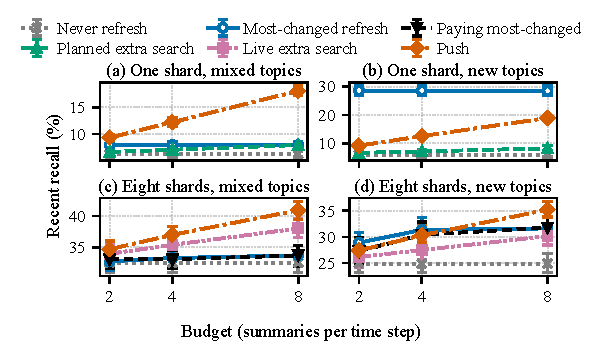
\includegraphics[width=\columnwidth]{figures/fig_budget.pdf}
\caption{Recent recall at each budget, at \RNumPlainQueriesDefault{} queries per time step. Top: one-shard placement, where all refresh rules tie and only planned extra search was run. Bottom: eight-shard placement, with live extra search and paying most-changed (Section~\ref{sec:follow}); most-changed is the best refresh rule there, except that largest-shard is slightly higher at a budget of two on mixed topics. Vertical lines show each method's own \RNumCIPct{} range. Table~\ref{tab:main} compares methods query by query, so it can show a clear difference even where these ranges overlap. Vertical scales differ.}
\label{fig:budget}
\end{figure}

\subsection{One-Shard Placement: The Topics Decide}
\label{sec:res-one}

When one shard takes all of a time step's new passages, all five refresh rules matched refresh all on every query, as predicted.
So the registered probe test could not pass on the new-topic stream.
It was skipped on the mixed-topic stream, where refresh all missed the \RNumPlainGateThreshold{}-point threshold.
Since only one shard changes, the four rules other than the probe spend the rest of each budget re-sending unchanged summaries.
That is \RNumMTwoUnmodShareBTwo{} of a budget of two and \RNumMTwoUnmodShareBEight{} of a budget of eight.

On the mixed-topic stream, never refresh finds \RNumPlainLvlMTwoNRSteady{} of recent matches, about what chance gives when two of \RNumNumShards{} shards are searched.
Refresh all raises this only to \RNumPlainLvlMTwoAFSteady{}, and it lowers overall recall by \RNumPlainGateMTwoOverallSteady{} points, with a drop in every seed.
Plausibly, \RNumCentersPerSummary{} centers cannot describe a shard that holds a mix of every topic.
Push wins at every budget (Fig.~\ref{fig:budget}a), so the registered test that refresh beats both alternatives failed on this stream.
Push keeps \RNumMTwoPVShareBTwo{} to \RNumMTwoPVShareBEight{} of new passages across budgets, and its gain over never refresh closely matches what that share predicts.

On the new-topic stream, the result reverses.
There, each time step's passages come from one or two new clusters, which \RNumCentersPerSummary{} centers describe well.
Refresh all raises recent recall from \RNumPlainLvlMTwoNRNewTopic{} to \RNumPlainLvlMTwoAFNewTopic{}.
Refresh beats push at every budget, but its lead shrinks from \RNumPlainHFourPVBTwoNewTopic{} points at a budget of two to \RNumPlainHFourPVBEightNewTopic{} at eight.
Larger budgets push more passages, while \RNumOneSummary{} fresh summary per time step is already enough.
Refresh also beats planned extra search at every budget, by \RNumPlainHFourESMinNewTopic{} to \RNumPlainHFourESMaxNewTopic{} points, so the registered test passed on this stream.

\subsection{Eight-Shard Placement: Close Calls}
\label{sec:res-eight}

When eight shards share each time step's new passages, more shards change than the smaller budgets can refresh.
On the mixed-topic stream, refresh all again gains little, \RNumPlainGateMThreeSteady{} points, and lowers overall recall by \RNumPlainGateMThreeOverallSteady{} points, with a drop in every seed.
Push beat refresh at every budget, and so did live extra search (Fig.~\ref{fig:budget}c).
On the new-topic stream, refresh all gains \RNumPlainGateMThreeNewTopic{} points and passes the \RNumPlainGateThreshold{}-point threshold on average.
In one seed, though, it gained only \RNumPlainGateMThreeMinSeedGap{} points.
The best two shards per query, chosen as in Section~\ref{sec:res-near}, would find \RNumPlainOracleMThreeSteadyPct{} of recent matches on mixed topics, against \RNumPlainLvlMThreeBFourAFSteady{} for refresh all.
On new topics they would find \RNumPlainOracleMThreeNewTopicPct{}, against \RNumPlainLvlMThreeBFourAFNewTopic{}.

On new topics at a budget of two, most-changed, the best refresh rule, leads push by \RNumPlainHFourBPVBTwoNewTopic{} points, but the lead is fragile.
Its range starts at only \RNumPlainHFourBPVBTwoNewTopicLow{} points, one seed favors push, the simpler test includes zero, and it relies on free score bytes (Section~\ref{sec:follow}).
At a budget of four neither clearly wins, and at eight push wins by \RNumPlainHFourBPVBEightNewTopic{} points (Fig.~\ref{fig:budget}d).
Most-changed also leads live extra search on new topics at every budget, but only the lead at four is not fragile.
At two, one seed favors live extra search and the lead relies on free score bytes; at eight, the simpler test includes zero.
So the registered test that refresh beats both alternatives failed at every budget on mixed topics.
On new topics it passed only at a budget of two, and that pass is fragile.

On overall recall, which also counts older matches, live extra search beat push at every budget, on both streams, by \RNumPlainESOPVOverallMin{} to \RNumPlainESOPVOverallMax{} points.
It also beat refresh there on new topics at budgets of four and eight.

On new topics, push beats never refresh by about \RNumMThreePVNewTopicExcessMin{} to \RNumPlainPVExcessMax{} points more than its share of new passages predicts.
Plausibly, this is because push keeps each time step's last passages, which on this stream tend to come from the newest cluster.
The planned version of extra search was at most \RNumPlainLookaheadMThreeMax{} points ahead of the live one here.
The live version spent slightly less than its budget, as little as \RNumMThreeESOShareOfRefreshBTwoNewTopic{} of it.
That shortfall, worth only about \RNumMThreeESOUnderspendValMin{} to \RNumPlainESOUnderspendMax{} points, changes no winner but blurs how much of the planned lead comes from planning ahead.

\subsection{Which Shards Should Refresh?}
\label{sec:res-which}

We expected the probe to beat each other rule by at least \RNumPlainGateThreshold{} points, but it did not.
In eight-shard placement on new topics at a budget of four, most-changed found \RNumPlainHThreeBRNMinusDCNewTopic{} points more recent matches than the probe (Table~\ref{tab:main}).
The probe showed no clear difference from most-searched or largest-shard.
It clearly beat only rotation, which itself did no better than never refresh at budgets of two and four.
Against most-searched, all five seeds and the simpler test favored the probe, but our range, wider here (Section~\ref{sec:stats}), included zero.
On mixed topics the probe test was skipped, because refresh all missed the \RNumPlainGateThreshold{}-point threshold.
At a budget of eight, the four rules other than the probe refreshed all eight open shards, matching refresh all on every query as predicted.
The probe refreshed seven and on average trailed refresh all by \RNumPlainPredRNBEightNewTopic{} points on new topics.
On mixed topics it trailed by \RNumPlainPredRNBEightSteady{} points, with no clear difference.

The probe's estimate was often zero for every shard.
That happens when no sample query would both move a shard into its top two and find a new passage among its \RNumPlainTopK{} best matches.
In eight-shard placement at a budget of four, this happened in \RNumSpearmanZeroPctNewTopicMThree{} of time steps on new topics and \RNumSpearmanZeroPctSteadyMThree{} on mixed topics.
Under starting-center placement on the mixed-topic stream, its estimate was zero for every shard in \RNumSpearmanZeroPctSteadyMOne{} of time steps.
The probe then falls back to shards over the waiting limit first, then the lowest shard number.

To see which signal points to the shards worth refreshing, we measure each shard's benefit in each time step.
The benefit counts the test queries' true best matches that would move into the two searched shards if that shard alone sent a fresh summary.
It counts old and new matches and does not subtract matches that would drop out.
We rank the \RNumNumShards{} shards by this benefit and by a signal, and compare the two rankings with Spearman's rank correlation.
Like two judges ranking the same contestants, it is one when they agree exactly, near zero when unrelated, and minus one when reversed.
We average it over the time steps in which both the benefit and the probe's estimate differ between shards, and then over the five seeds.
Skipping the steps where the probe cannot tell shards apart favors the probe, and the averages have no ranges.
In eight-shard placement on new topics at a budget of four, the probe's estimate scored \RNumSpearmanRNNewTopicMThree{}, measured on the runs that used the probe.
A plain count of each shard's new passages scored \RNumSpearmanNewVecsNewTopicMThree{}.
Unlike most-changed, the count ignores how far the new passages lie from the old centers, and we did not measure most-changed this way.
On average, the count scored higher in every starting-center and eight-shard setting.
It is free only if the coordinator tracks how many passages each shard receives.

\subsection{Follow-Up: When Most-Changed Pays for Its Scores}
\label{sec:follow}

The follow-up charges most-changed for its own score messages.
Paying \RNumDCScoreEpochBytes{} bytes per time step costs it a whole summary and leaves \RNumAddThreeDCUnspentEpochBytes{} bytes of each step's budget unused.
This is a pessimistic case for most-changed, because unused bytes do not carry over, and we did not run a version where they do.
If unused bytes carried over, its \RNumDCScoreEpochBytes{} bytes per step would add up to less than one summary over a \RNumNumEpochs{}-step run.

Paying most-changed refreshes as many summaries as the probe, so comparing the two shows which picks better shards.
Of most-changed's \RNumPlainHThreeBRNMinusDCNewTopic{}-point lead over the probe in the main runs, at a budget of four on new topics, \RNumPlainXOneRNBFourNewTopic{} points remained.
The other \RNumPlainXThreeDCBFourNewTopic{} points came from the summary that the probe's messages cost it.
At a budget of eight, paying most-changed led by \RNumPlainXOneRNBEightNewTopic{} points.
All \RNumAddThreeXOnePosSeedsBFourBEight{} seed results at these two budgets favored it.
At a budget of two on new topics, \RNumPlainXThreeDCBTwoNewTopic{} of the probe's \RNumPlainRNLossBTwoNewTopic{}-point main-run loss came from the lost summary.
That part is fragile, because the simpler test includes zero.
At that budget, and on mixed topics, the two rules showed no clear difference.
This comparison still favors the probe, which sends \RNumAddThreeRNExtraEpochBytesVsChargedDC{} more bytes per time step and keeps its setup broadcast free.
At a budget of four on new topics, paying most-changed led by \RNumPlainXOneAllZeroGap{} points in steps where the probe's estimate was all zero.
In the other steps it led by \RNumPlainXOneNonZeroGap{}.
There, the waiting limit forced \RNumAddThreeRNForcedSumBFourNewTopic{} of the probe's \RNumAddThreeTotalRefreshesBFour{} refreshes.
It forced \RNumAddThreeChargedDCForcedSumBFourNewTopic{} of the \RNumAddThreeTotalRefreshesBFour{} made by paying most-changed.

Against push on new topics, paying most-changed lost the fragile lead that most-changed had at a budget of two.
Push was then \RNumPlainXTwoPVBTwoNewTopic{} points ahead, with no clear difference, so this is not a win for push either.
At a budget of four there was still no clear winner, and at eight push led by \RNumPlainXTwoPVBEightNewTopic{} points.
Against live extra search on new topics, paying most-changed had no clear lead at a budget of two and a clear lead at four.
At eight its lead was fragile, because one seed pointed the other way.
On overall recall, live extra search led it on new topics at budgets of four and eight, though at four the simpler test includes zero.
On mixed topics, push and live extra search each led paying most-changed at every budget.
At a budget of eight, paying most-changed refreshes seven summaries, so it no longer matches refresh all on every query.
On new topics it differs from unpaid most-changed by only \RNumPlainXThreeDCBEightNewTopic{} points, with no clear difference.

The follow-up also reran starting-center placement at \RNumPlainQueriesHigh{} queries per step, where most-changed had overtaken extra search on new topics.
Paying most-changed still edged planned extra search there, by only \RNumPlainXFourESNewTopic{} points.
That lead is fragile: its range barely clears zero, and it touches zero when we redo the resampling with other random draws.
It also comes only from the first \RNumPlainXFourEarlySteps{} of the \RNumNumEpochs{} time steps.
Planned extra search was \RNumPlainXFourLateGap{} points ahead in later steps and \RNumPlainXFourOverallGap{} ahead on overall recall, with no clear difference there.
Paying most-changed also led live extra search by \RNumPlainXFourESONewTopic{} points, with a range starting at \RNumPlainXFourESONewTopicLow{}.
Push still beats paying most-changed there, by \RNumPlainXFourPVNewTopic{} points.
